\documentclass{beamer}


\usepackage[utf8]{inputenc}
\usepackage{pgfpages}
\usepackage{xcolor}

\setbeameroption{show notes}
\setbeamertemplate{note page}[plain]
\setbeameroption{show notes on second screen=left}

\usetheme{Warsaw}
\graphicspath{ {./images/}{../images/}{../kcov-swedencpp/images/}{../../kcov-swedencpp/images/}{output/} }

\AtBeginSection[specialframe]
{
  \begin{frame}{Table of Contents}
   \tableofcontents[currentsection]
  \end{frame}
}

\title[What's in a binary?] %optional
{What's in a binary?}

%\subtitle{A short story}

\author{Simon Kågström}

\institute
{
  Consultant\\
  \texttt{https://github.com/SimonKagstrom/emilpro}
}

%\logo{\includegraphics[height=1.5cm]{lion-logo.png}}

\begin{document}

\begin{frame}
  \titlepage
  \note{
    My name is Simon Kågström and I work as a consultant, currently at Profoto. Tonight I will present
    emilpro, which is a graphical disassembler.
  }
\end{frame}



\begin{frame}{Background}
  \begin{itemize}
    \item I have a few themes that I often return to in my projects
    \item One of these is disassembly
  \end{itemize}
  \note{
    I don't know about you, but at least I tend to return to a few themes over and over again.
    These projects are never finished, and rarely really working, but they are fun to work on.

    For some of these, I've done multiple reimplementations, and the topic of this talk is one
    of them. This is actually the third implementation, the first one was started almost 20 years ago
    now as a Python application called Dissy. You get a sense of how old I am now, I guess!

    That one really just parsed objdump output, so after a few years I thought I could do better,
    and rewrite it in C++ and use libraries for the parsing instead. So a bit over 10 years ago, I
    rewrote it as "emilpro", which is a pun on IDA pro which at least then was the state of the art.

    It was sort of working, but bitrotted and a few years later it wasn't even possible to compile
    anymore. But when I again needed disassembly this year, I thought I'd just rewrite it again
    and that's the topic of this talk. The third implementation now, and counting!
  }
\end{frame}


\begin{frame}
  \frametitle{Demo}
  \note{
    I'll start with a small demo of the application.
  }

  
\includegraphics[width=\linewidth]{kalkyl}
  % Start the app. Show symbols, filtering, cross-reference, jump lanes, address history
\end{frame}

\begin{frame}
  \frametitle{Outline}
    \begin{itemize}
      \item Part I: Motivation
      \item Part II: What does the disassembly writer need?
      \item Part III: Why is this easier now than 10 years ago?
    \end{itemize}
  \end{frame}

\begin{frame}{Part I: Motivation}
\end{frame}

\begin{frame}[fragile]{Motivation}
  \begin{itemize}
    \item C/C++ with inline assembly
    \item Systems and programming environments where a debugger wasn't available
  \end{itemize}
  \begin{Example}
    \begin{semiverbatim}
      \scriptsize
\#define \_syscall1(type,name,atype,a) type name(atype a) \{
        unsigned long out;
        \_\_asm\_\_ volatile (
        ".set  push\\n.set  noreorder\\n"
        ".short 0xfefe\\n"
        ".short \%1\\n"
        ".pushsection .cibylstrtab, \\"aS\\"\\n"
        "1: .asciz \\"" \#name "\\"\\n"
        ".popsection\\n"
        ".long 1b\\n"
        ".set\\tpop\\n"
        "move \%[out], \$2\\n
        : [out]"=d" (out)
        : "r"(a)
        : "memory", "\$2"
        );
        return (type) out;
\}
    \end{semiverbatim}
  \end{Example}

  \note{
    I've during my career, although mostly for non-work related tasks, multiple times had to rely on
    diassembly for debugging and understanding how things work while working on low-level stuff.

    Back in the days, I was also writing a lot of inline assembly, and side effects of that is easy
    to get almost correct, so that it breaks in subtle ways when more complex code is used. If you've
    used GCC inline assembly, you'll know that it's quite powerful but it's very important to correctly
    specify input, output correct, as well as side-effects, which are known as clobbered. I had to
    look the word up by the way, and clobbered means "to hit someone or something hard and repeatedly".
    That summarizes GCC inline assembly well, I think!

    In some instances, I had no way of debugging the code, but could get backtraces and register dumps.
    The disassembly was then the only way to figure out what was going on.
  }
\end{frame}

\begin{frame}{Backstory}
  \begin{itemize}
    \item Objdump output is cumbersome to navigate through
    \item I wanted a graphical application that allows easier navigation
  \end{itemize}
  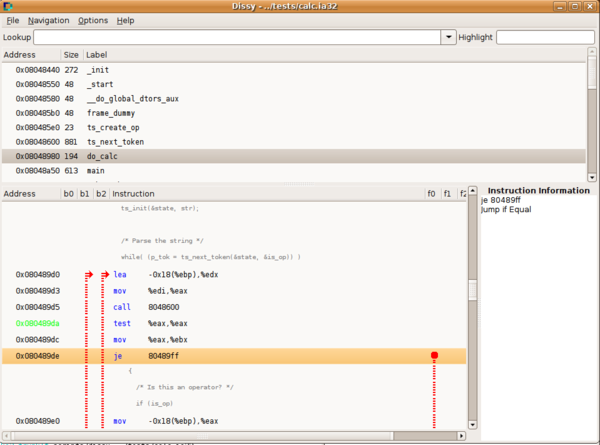
\includegraphics[width=4.5cm]{dissy-with-instruction-box-600}
  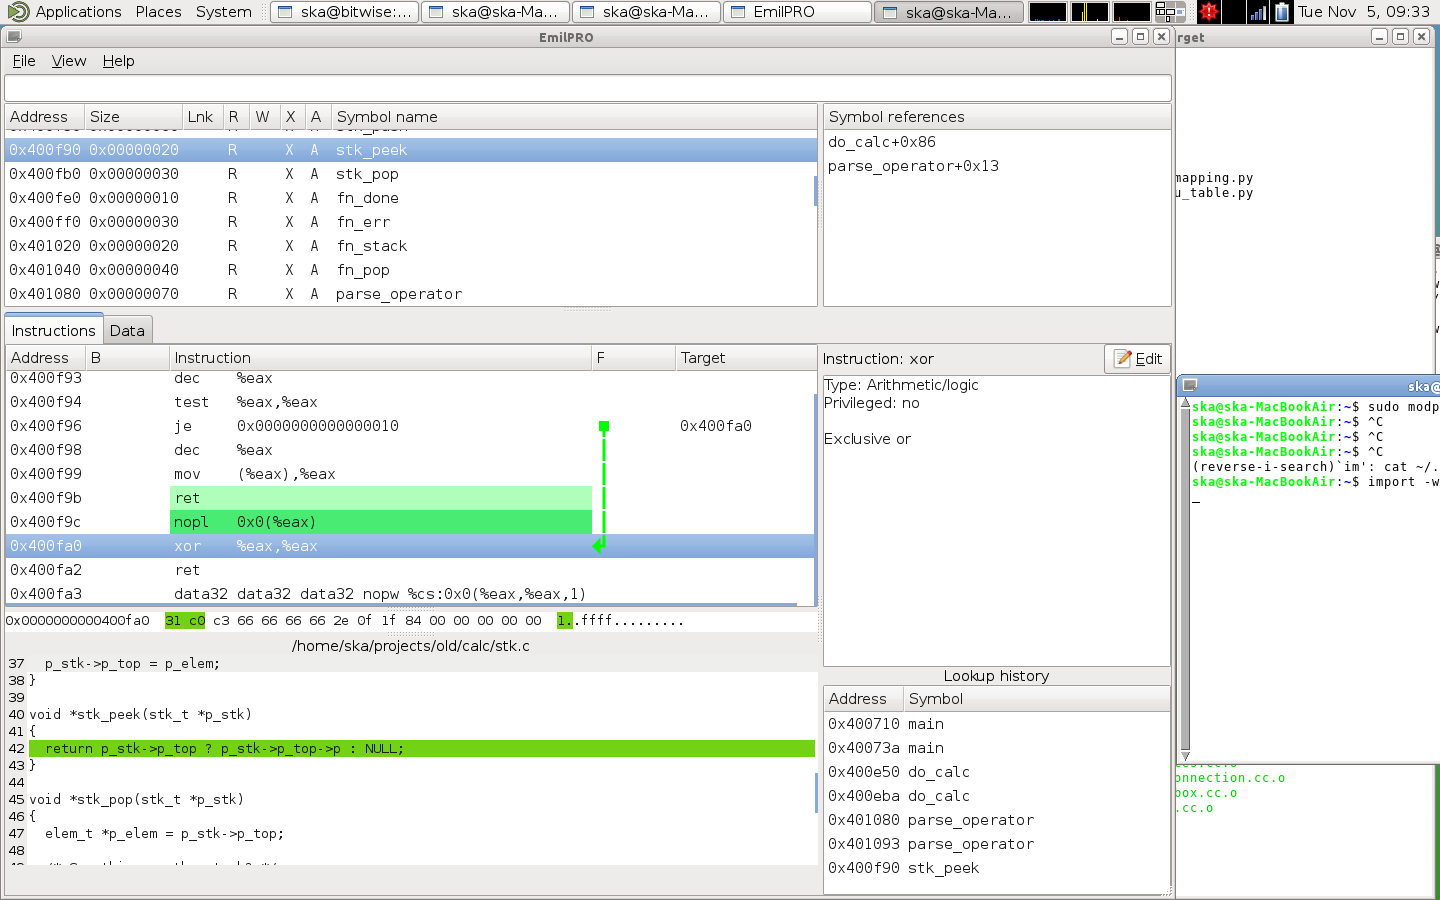
\includegraphics[width=6cm]{old_emilpro}
  \note{
  Using plain Objdump for this is very cumbersome, so I wanted an easier way to navigate the
  disassembly.
}
\end{frame}

\begin{frame}{Part II: What is needed for a disassembler?}
\end{frame}


\begin{frame}{Binary formats}
  \begin{itemize}
    \item \textbf{Linux/FreeBSD} etc: ELF
    \item \textbf{MacOS}: Mach-O
    \item \textbf{Windows}: PE
  \end{itemize}
    % ELF + DWARF
    % Mach-O
    % PE
    % The three rules for an instruction set architect
    \note{
      The binary format is used for executables and linkable object files. These are the
      three probably most commonly used formats today.

      ELF is used for Linux, FreeBSD and others, but also as an intermediate format for a
      lot of embedded systems. MacOS uses the Mach-O format, from the Mach microkernel. You'll
      notice here that the binary format engineers have a sense of humor, and you also have
      the DWARF debugging format to go with ELF and also Mach-O. If you invent a new format,
      I'd suggest ORC as a name.

      The execption to the funniness is Windows, which simply calls their format pee.

      I believe MS-DOS uses the COFF format.

      The job description for an instruction set architect
      \begin{itemize}
        \item You should create an instruction set which consists of abbreviations of
        common words for no particular reason. Bonus point for using unclear meanings
        (for example MOV, which is an abbreviation of "move", but actually copies the
        value)
        \item Your instruction set should be basically MIPS, but with a few improvements.
        Sometimes "improvements".
        \item Your instruction set should contain at least one funny sounding instruction.
        Case in point: EIEIO.
      \end{itemize}
    }

    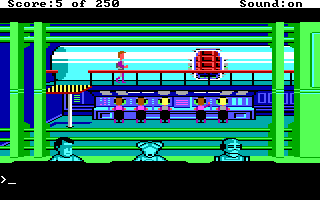
\includegraphics[width=7cm]{sq2_computer_room}
  \end{frame}


\begin{frame}{How to write a dissassembler?}
  \begin{columns}
    \begin{column}{0.5\textwidth}
      I did not write everything from scratch!

      \begin{itemize}
        \item \textbf{libbfd}: Part of binutils, used for reading binary files
        \item \textbf{capstone}: Disassembler library
        \item \textbf{Qt}: GUI framework
      \end{itemize}
    \end{column}
    \begin{column}{0.5\textwidth}
      \includegraphics[width=5cm]{emilpro_structure}
    \end{column}
  \end{columns}
  \note{
    I didn't write everything from scratch.

    It's like Newton said: "If I hadn't been standing on the shoulders of giants, I wouldn't have reached
    the apple."

    The three main building stones are Qt, the GUI framework, libbfd and capstone. libbfd reads binary files
    to gather symbols, relocations and instruction data which the disassembler then picks up. The sectiond
    data, for text sections are then fed to capstone, which disassembles it into instructions.
  }
\end{frame}

  \begin{frame}{Loading a binary}
    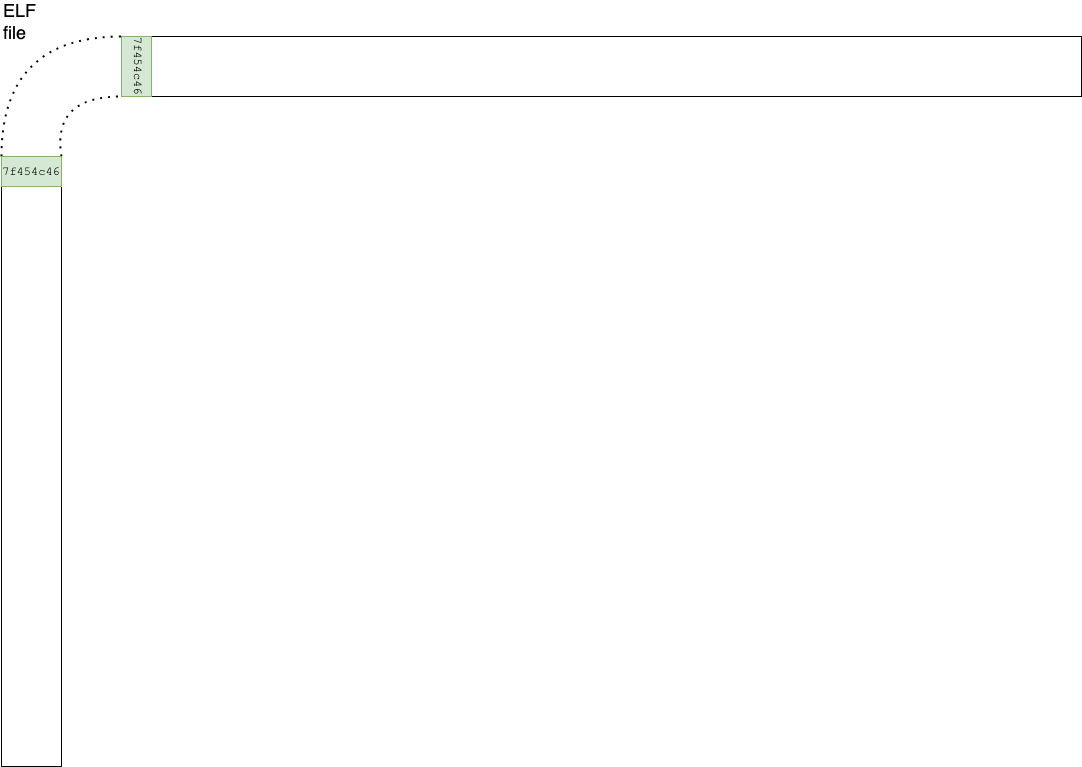
\includegraphics[width=8cm]{elf_background}
  \end{frame}

  \begin{frame}{Loading a binary, sections}
    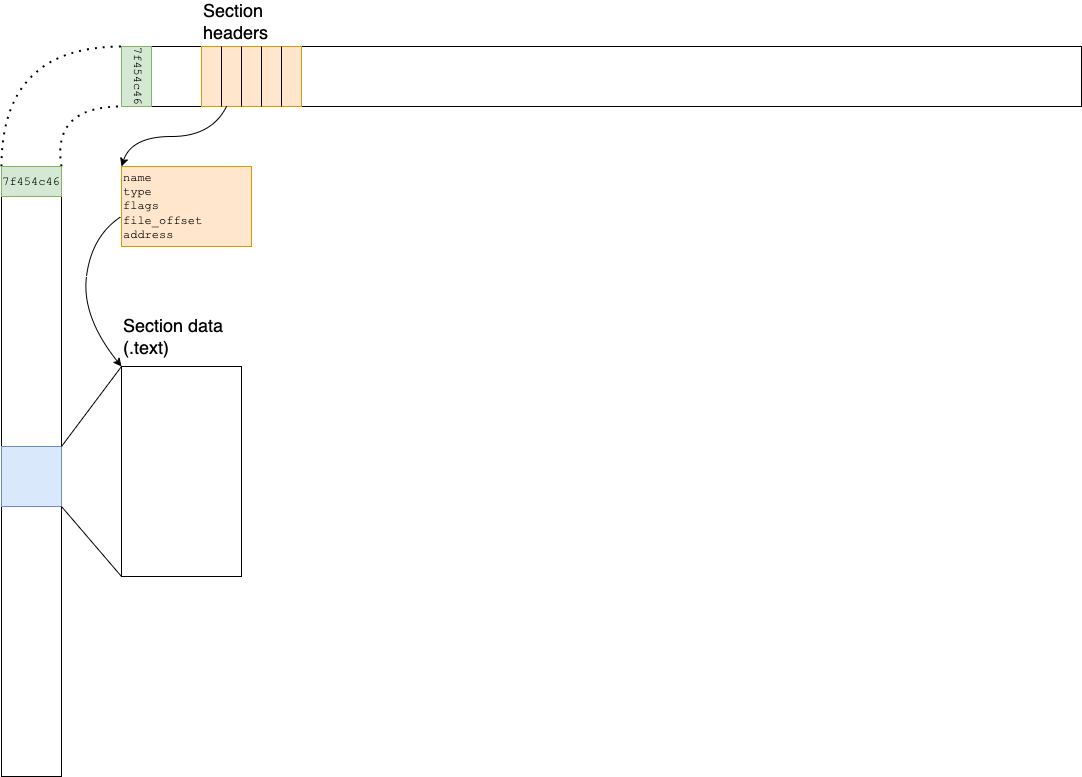
\includegraphics[width=8cm]{elf_sections}
  \end{frame}

  \begin{frame}{Loading a binary, symbols}
    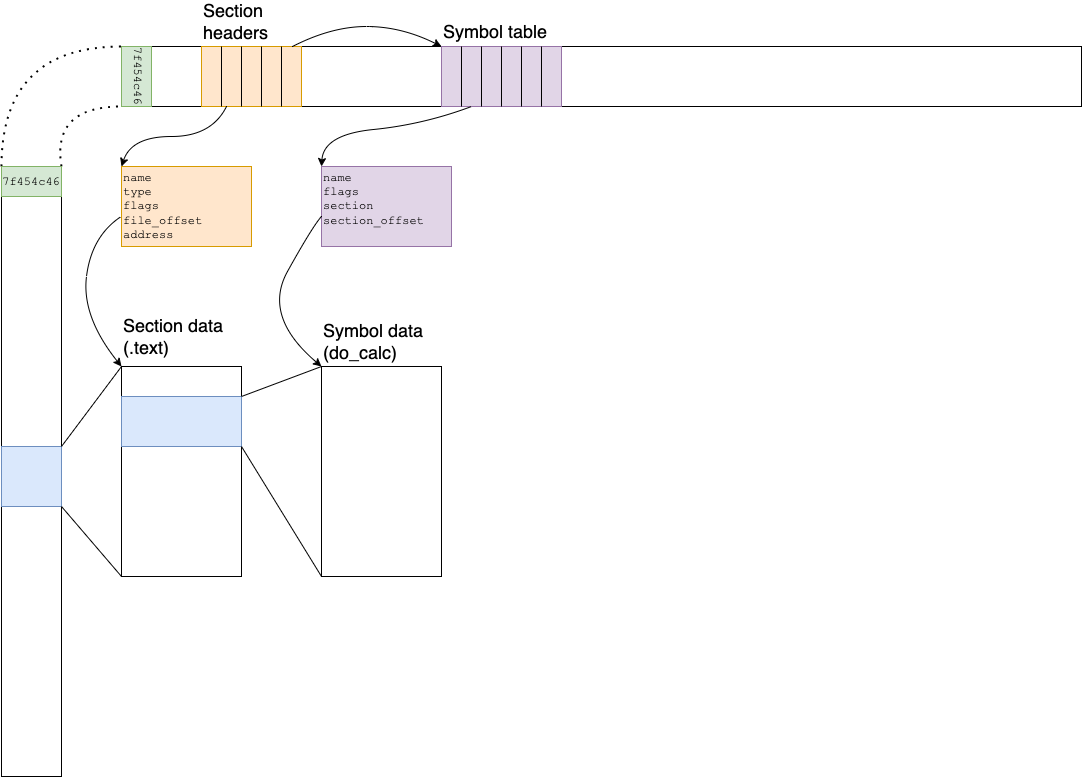
\includegraphics[width=8cm]{elf_symbols}
  \end{frame}

  \begin{frame}{Loading a binary, instructions}
    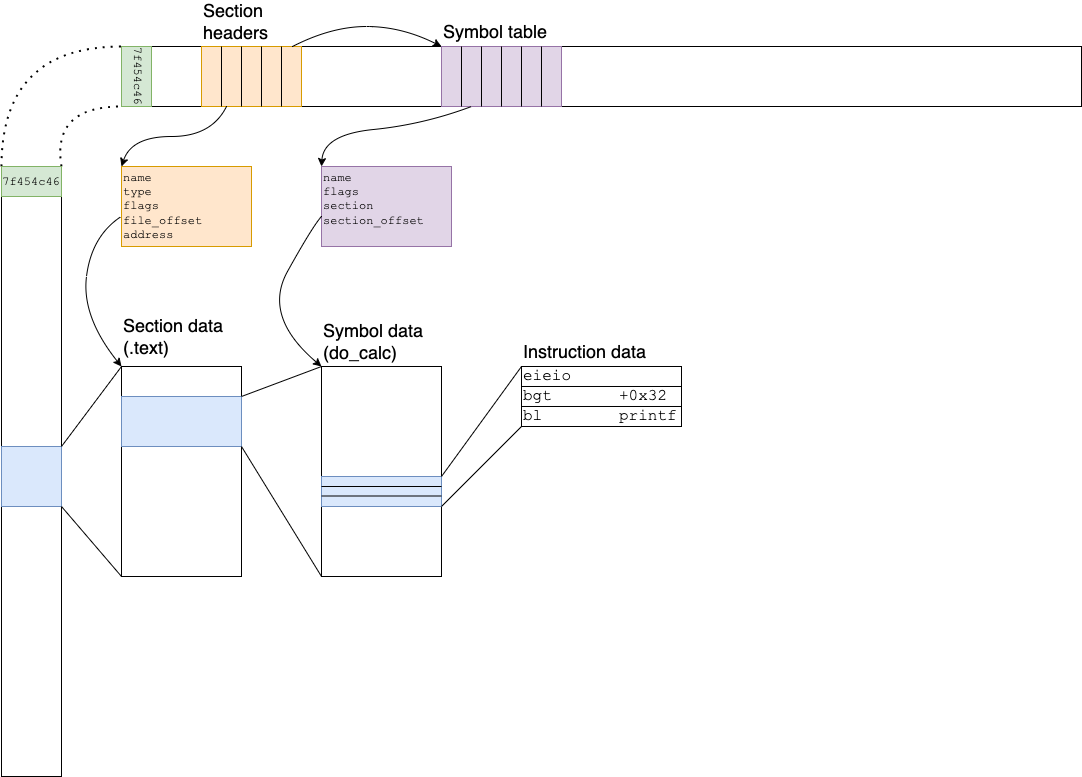
\includegraphics[width=8cm]{elf_instructions}
  \end{frame}

  \begin{frame}{Loading a binary, relocations}
    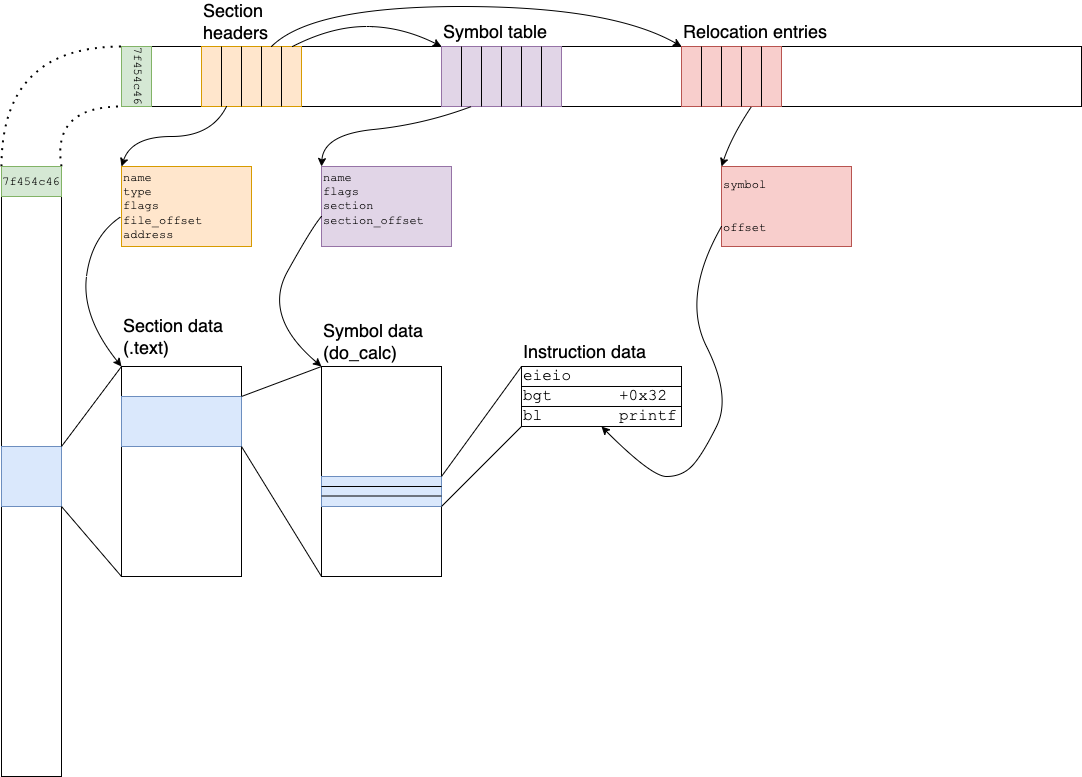
\includegraphics[width=8cm]{elf_relocations}
  \end{frame}

  \begin{frame}{Loading a binary, relocations}
    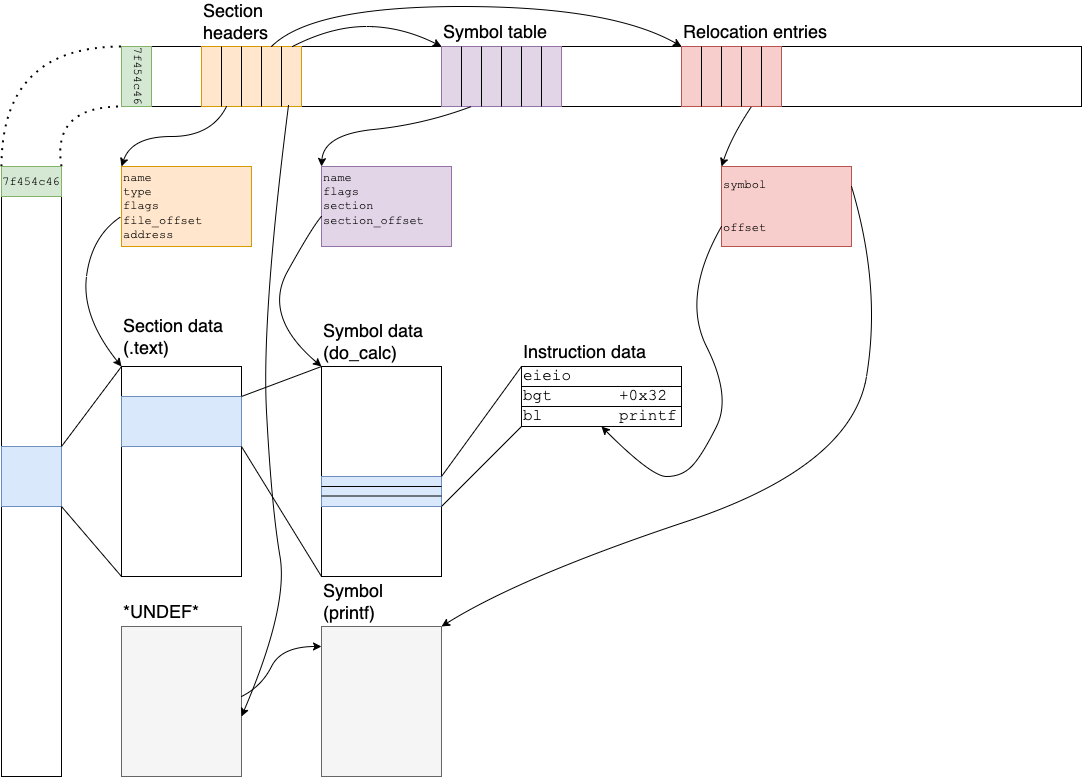
\includegraphics[width=8cm]{elf_undefined_section}
  \end{frame}

  \begin{frame}{Actors and objects}
    Actors
    \begin{itemize}
      \item \textbf{Compiler}
      \item \textbf{Linker}
      \item \textbf{Loader}
      \item \textbf{Disassembler}
    \end{itemize}
    Objects
    \begin{itemize}
      \item \textbf{Instructions}: The actual code
      \item \textbf{Sections}: Text, data, debug info etc
      \item \textbf{Symbols}: Functions/methods, variables, ...
      \item \textbf{Relocations}: Call sites for later resolving
    \end{itemize}
    % What is compiler, linker, loader?
    % Show in emilpro

    % Sections, symbols, relocations
    % Disassembler, compiler, linker, loader
\end{frame}

\begin{frame}{Producing a binary}
  \begin{columns}
    \begin{column}{0.5\textwidth}
      The compiler produces symbols, relocations plus data and text sections
    \end{column}
    \begin{column}{0.5\textwidth}
      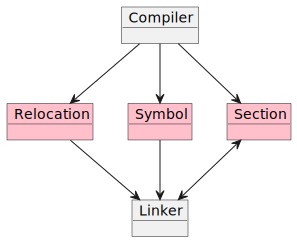
\includegraphics[width=5cm]{compiler_linker}
    \end{column}
  \end{columns}
  % Sumbol example from ELF (dump reloc)
\end{frame}

\begin{frame}{Relocations}
  \begin{itemize}
    \item If a non-local function is called, an undefined symbol is added
    \item The compiler adds a relocation entry for the call site
    \item When linking, the linker will resolve these symbols
    \item Different types depending on instruction
  \end{itemize}

  % Example from ELF (dump reloc)
\end{frame}

\begin{frame}{Loading a binary}
  Different categories of binaries are handled differently:
  \begin{itemize}
    \item Execute from direct-mapped flash (embedded systems)
    \item Static executables
    \item Dynamic executables
    \item PIEs (Position-Independent Executables)
  \end{itemize}

  % Sections, symbols, relocations
  % Example from embedded system
  % Load sections into memory
  % Entry point
  % Disassembler, compiler, linker, loader
  \includegraphics[width=7cm]{loader}
\end{frame}

\begin{frame}{Static executables}

\end{frame}

\begin{frame}{Dynamic executables}
  % Global offset table (for global data, ignored here)
  % Procedure linkage table (for function calls)
  % Relocation entries are for the PLT, not the call sites
  % - when a function is called, it's called through the PLT
  % - the relocated PLT jumps to the function in the shared library
  % - at least Linux handles PLT resolving lazily, i.e., only when the
  %   function is called
\end{frame}

\begin{frame}{PIEs}
    % Relocation entries
    % Why are they needed?
\end{frame}

\begin{frame}{libbfd}
    %Example from documentation

    \note{
      libbfd is part of binutils, so is shipped with the linker.
    }
  \end{frame}

\begin{frame}{Part III: Why is this easier now than 10 years ago?}
  %move from binutils
  %c++11+
  %conan
  %copilot
\end{frame}


\begin{frame}{Bad design decisions in the original project}
  \begin{itemize}
    \item libbfd for disassembly: the multiarch-dev issue
    \item feature creep: core functionality sketchy, work on irrelevant features
  \end{itemize}

  % built my own binutils. Bitrot and was unbuildable later
\end{frame}

\begin{frame}{C++20 and infrastructure}
  \begin{itemize}
    \item The previous implementation was done just around the C++11 introduction, but used C++03
    \item Now C++23, so much better!
    \item Conan and ASAN

    % example of c++03 vs c++23

    % binutils

    % The main reason for my previous failure was the libbfd rebuild
    % conan allows newer versions than in the distribution, and the same between os:es.
    % maybe not so good for distributions though.

    % Conan libiberty helps with MacOS libbfd linking.
  \end{itemize}
\end{frame}

\begin{frame}{AI}
  \begin{itemize}
    \item I use Github copilot
    \item Very helpful with Qt development
  \end{itemize}
  % Unit test example (drawing, ugly)
  % LaTeX example (bad)
  % Qt example (good)
  %copilot

\end{frame}



\begin{frame}{Questions and comments!}
  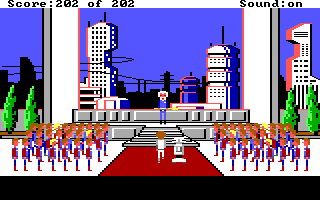
\includegraphics[width=\linewidth]{sq_final}

  Images from \url{http://www.falselogic.net/LetsPlay/SpaceQuest.html}

  Ian Lance Taylors linker series is the source of parts of this talk
  \url{https://www.airs.com/blog/index.php?s=Linkers}

  \note{
  First I have a teaser for my next talk. Do we have any people living or working in
  Uppsala here? Do you know that you live in the edge case?
  }
\end{frame}

\end{document}
